% --- 1. INTRODUCTION ---
\section{Introduction}
\label{sec:intro}

Kidney diseases, encompassing both neoplastic formations (such as renal cell carcinoma) and non-neoplastic conditions (such as nephrolithiasis and complex cysts), represent a mounting global health challenge. Precise and timely diagnostic workflows are critical for patient survival and effective surgical intervention. Traditionally, the identification, staging, and volumetric analysis of these pathologies have relied almost exclusively on the manual inspection of Computed Tomography (CT) and Magnetic Resonance Imaging (MRI) scans by expert radiologists. This conventional paradigm is inherently subjective, highly time-consuming, and susceptible to inter-observer variability, particularly when differentiating subtle malignant subtypes or delineating complex, multi-focal tumor boundaries for partial nephrectomies.

In recent years, the integration of deep learning (DL) into medical image analysis has fundamentally disrupted this diagnostic bottleneck~\cite{degadwala2024review}. DL architectures, specifically those engineered for advanced computer vision tasks, excel at extracting high-dimensional, non-linear semantic features from complex anatomical structures. While early computational applications in nephrology focused predominantly on binary classification (e.g., normal versus abnormal tissue), the current clinical frontier demands highly granular multi-class classification, exact 3D volumetric segmentation for preoperative planning, and robust algorithmic interpretability. A vast and accelerating body of recent literature has empirically validated the efficacy of these automated approaches across diverse clinical datasets, varying noise profiles, and different stages of disease progression~\cite{aljohani2025hierarchical, obaid2025noisy, khan2025multilevel, verma2025automated, rehman2024kidney, scales2012prevalence, wang2022survival, rajendran2025kidney}.

Despite accelerating algorithmic advancements, a critical translational gap remains between high-performing computational models and their actual deployment in clinical environments. Many contemporary models function as opaque "black boxes"~\cite{kadhim2024machine}, lacking the diagnostic explainability required to build trust among medical practitioners. Furthermore, diagnostic networks are frequently trained on narrow, homogeneous datasets, which severely limits their ability to generalize across diverse clinical hardware and disparate patient demographics.

This survey comprehensively synthesizes the methodologies, computational complexities, and clinical integrations of 63 recent DL frameworks. By meticulously analyzing the trajectory from traditional convolutional networks to advanced hybrid Transformer models, this paper aims to establish a clear taxonomy of current progress. Ultimately, we identify existing structural gaps and chart the necessary trajectory toward clinically viable, explainable AI (XAI) systems that integrate seamlessly into real-world renal care pipelines.

% --- 2. SURVEY METHODOLOGY ---
\section{Survey Methodology}
\label{sec:methodology}

To ensure a rigorous, transparent, and reproducible review of the current landscape, a systematic literature search was conducted following the Preferred Reporting Items for Systematic Reviews and Meta-Analyses (PRISMA) guidelines.

\subsection{Search Strategy and Selection Criteria}
The primary literature search was executed across major scientific databases, including IEEE Xplore, PubMed/MEDLINE, SpringerLink, and arXiv. The search was chronologically restricted to publications from the last five years to capture the most contemporary, state-of-the-art DL architectures. The core Boolean search string utilized combinations of the following keywords: ("Deep Learning" OR "CNN" OR "Transformer" OR "YOLO") AND ("Kidney Disease" OR "Renal Tumor" OR "Kidney Stone") AND ("CT Imaging" OR "Segmentation" OR "Classification" OR "Multi-class").

Initial screening yielded a substantial corpus of preliminary articles. These were subsequently evaluated against strict inclusion criteria: (1) empirical utilization of deep learning models on renal imaging modalities, (2) clear, quantitative reporting of performance metrics (e.g., Accuracy, Dice Similarity Coefficient, Intersection over Union), and (3) direct relevance to multi-class classification, volumetric segmentation, or surgical planning integration. 

\begin{figure}[htbp]
\centering
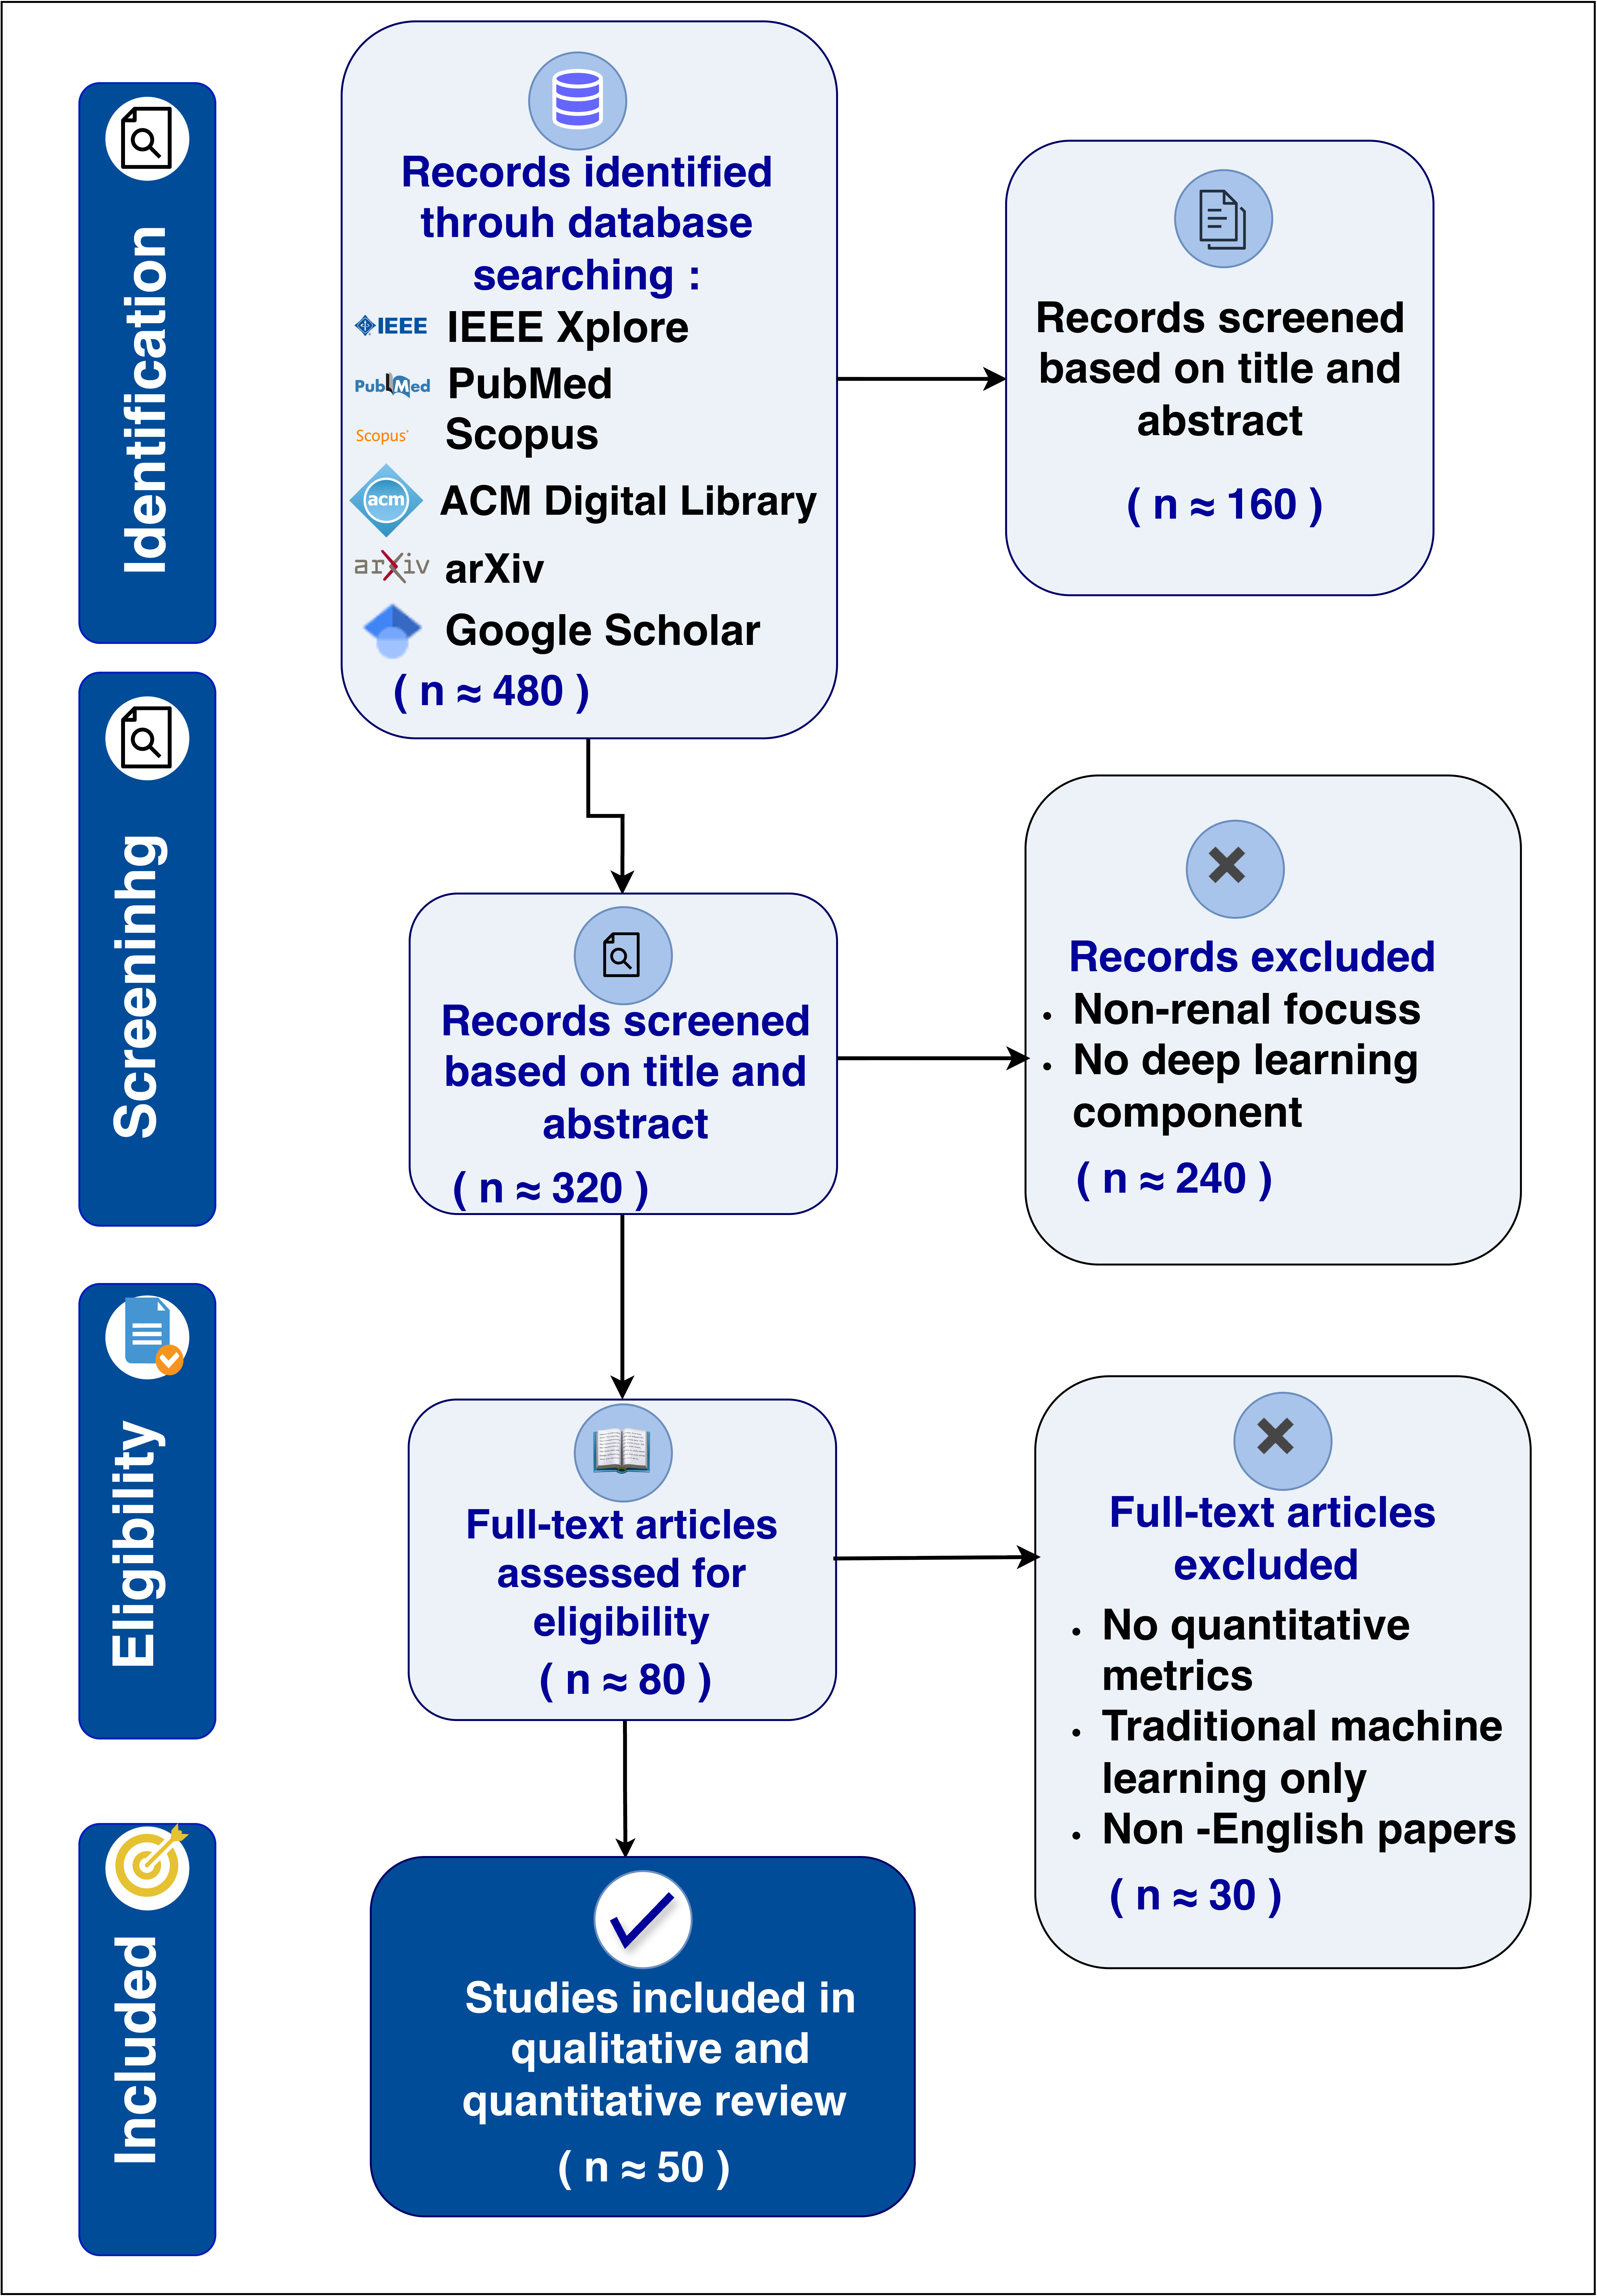
\includegraphics[width=\linewidth]{images/prisma_flow.png}
\caption{PRISMA flow diagram detailing the systematic literature search, screening, and selection process for the 63 included studies.}
\label{fig:prisma}
\end{figure}

\subsection{Data Extraction and Matrix Synthesis}
Following the removal of duplicates, non-peer-reviewed preprints lacking methodological rigor, and studies with insufficient computational detail, 63 primary papers were selected for deep extraction. For each study, data was systematically mapped into a comprehensive literature matrix. The extracted parameters include the imaging modality, primary pathology focus, dataset characteristics (e.g., benchmark challenge data versus proprietary clinical data), core model architecture, computational complexity, integration of Explainable AI (XAI), and identified deployment limitations.

\subsection{Identified Limitations in Current Literature}
Several persistent limitations that delay the seamless translation of computational models into real-world clinical environments are exhibited by the current literature on deep learning (DL) for renal disease diagnosis. In many contemporary architectures, diagnostic explainability is lacking, and these models are often regarded as opaque "black boxes"---a shortcoming that has been identified as a critical barrier to clinical adoption, since the trust of medical practitioners cannot easily be built without it~\cite{kadhim2024machine}.

Furthermore, significant feature limitations are found to persist across various modeling paradigms. In traditional machine learning approaches and hand-crafted feature descriptors (such as GLCM or ALBP), the semantic depth required to navigate the high variability of renal pathologies across diverse patient demographics is not achieved, and high sensitivity to imaging noise and low-resolution scans has been observed~\cite{farjad2021ct, hossain2024adaptive}. Conversely, although lightweight architectures are increasingly prioritized in order to reduce computational overhead and enable rapid, high-throughput triage, a loss of high-level semantic features is sometimes caused by the reduction in network layers in these models, and diagnostic precision is occasionally reduced after highly complex or multi-focal tumor presentations are encountered~\cite{bhandari2023lightweight, alqahtani2025kidneynext}.

Crucially, since narrow, homogeneous repositories are used to train a vast majority of frameworks, poor performance on unseen data is exhibited by several models. Severe performance degradation is frequently suffered when domain shifts are encountered caused by scanner heterogeneity, varying slice thicknesses, and vendor-specific HU calibrations across different hospital networks~\cite{aljohani2025hierarchical, abdelrahman2022deep, alzubi2022kidney, gao2026multitask}. This generalizability deficit is further exacerbated by a widespread lack of prospective clinical verification; in numerous research papers, static, public benchmark datasets are relied upon strictly, and no external multi-center validation or real-world clinical testing is conducted~\cite{liang2025multicenter, hossain2025detection, macin2025kidneynext, chen2023glunet, ye2026automated}.

Finally, single computational tasks---such as classification or segmentation---are frequently isolated by existing diagnostic pipelines, rather than holistic patient metadata and longitudinal clinical history being integrated, and overall utility in complex, real-world decision-making for surgical planning is thereby limited~\cite{liang2025multicenter, sreenivas2025enhancing}.

% --- 3. KEY DATASETS AND BENCHMARKS ---
\clearpage
\onecolumn % We switch to one column BEFORE the section title so the text and table stay together

\section{Key Datasets and Benchmarks}
The evolution of deep learning in renal imaging is intrinsically linked to the availability of large-scale, annotated datasets. Table \ref{tab:datasets} presents a synthesized breakdown of deep learning benchmarks, medical imaging cohorts, and textual corpora utilized across the reviewed literature, grouped categorically by data source. Figure \ref{fig:dataset_dist} illustrates the quantitative distribution of these datasets across the reviewed studies.

% --- Bar Chart Placed Immediately Below the Paragraph ---
\begin{figure}[h!]
\centering
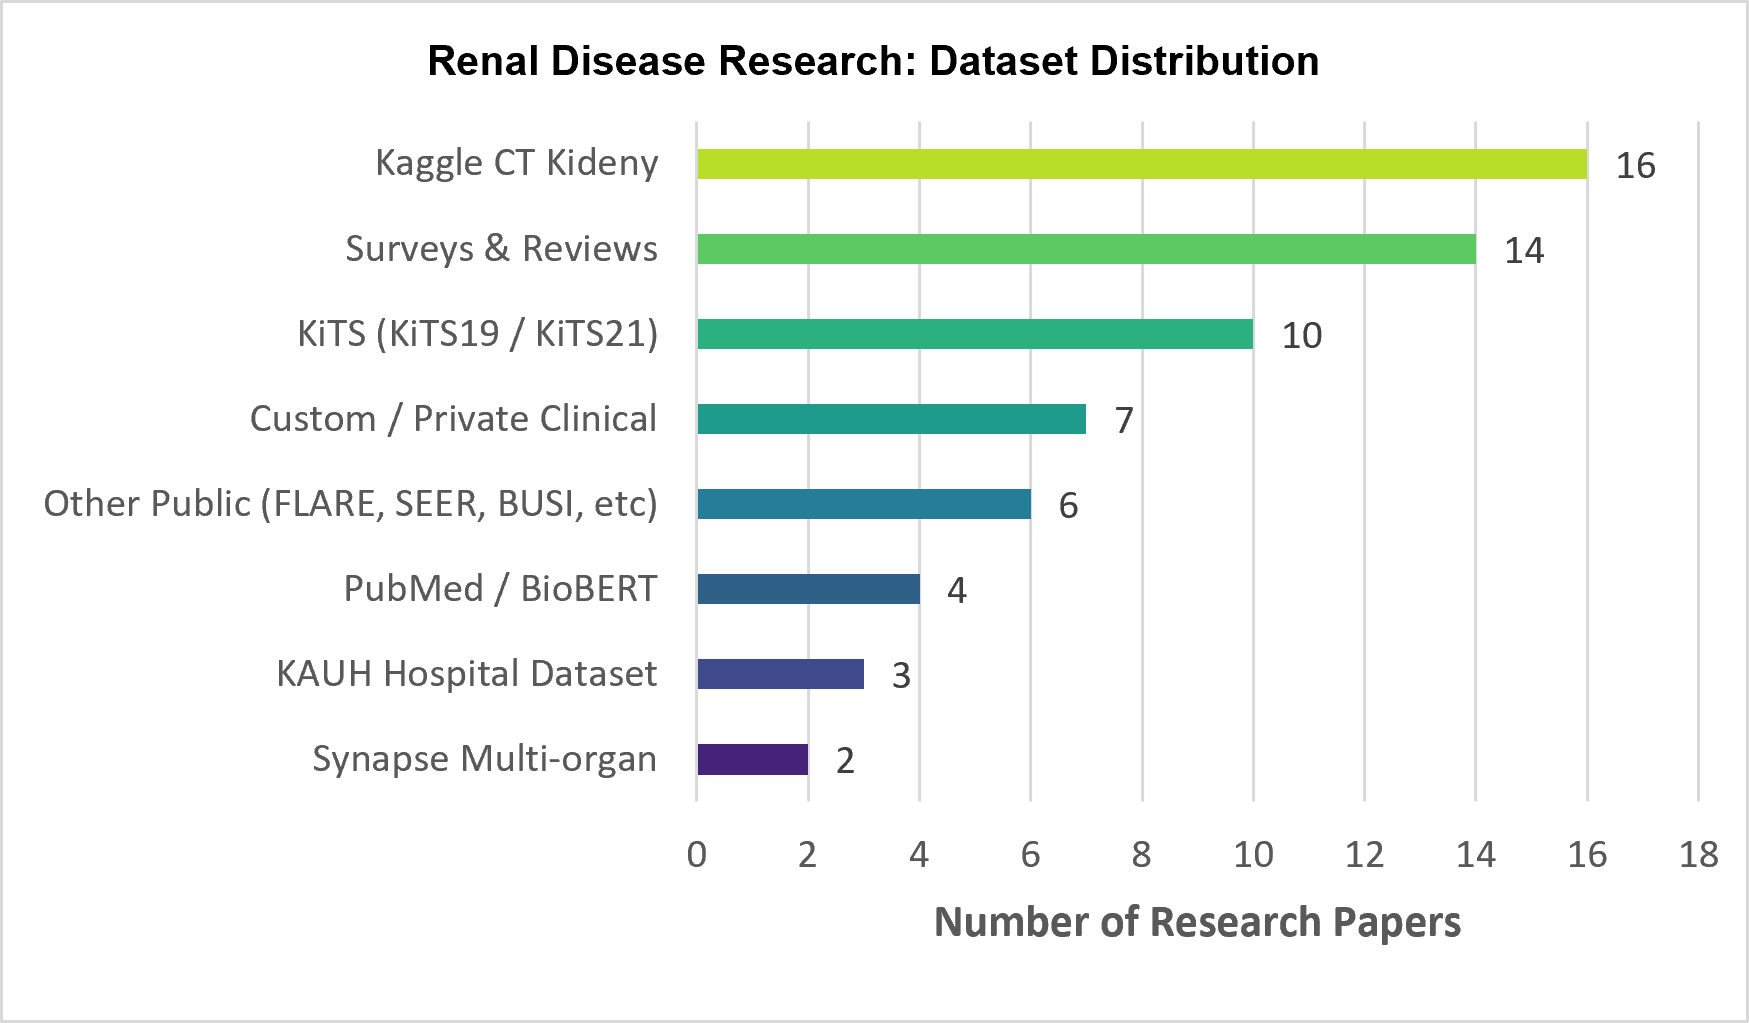
\includegraphics[width=0.85\textwidth]{images/dataset_distribution.png}
\caption{Quantitative distribution of datasets utilized across the reviewed renal disease research papers.}
\label{fig:dataset_dist}
\end{figure}

\vspace{1em} % Adds breathing room between the chart and the table

\renewcommand{\arraystretch}{1.5}  
\setlength{\tabcolsep}{4pt}          
\footnotesize                        

\begin{longtable}{|L{2.8cm}|L{1.8cm}|L{2.5cm}|L{3.0cm}|L{3.6cm}|L{2.2cm}|}
\caption{Summary of Reviewed Studies Grouped by Dataset (Papers 1--62)}
\label{tab:datasets} \\
\hline
\textbf{Dataset Name \& Link} & \textbf{Modality} & \textbf{Target Classes} & \textbf{Sample Size \& Breakdown} & \textbf{Performance Highlights} & \textbf{Utilizing Studies} \\
\hline
\endfirsthead

\multicolumn{6}{c}%
{{\bfseries \tablename\ \thetable{} -- continued from previous page}} \\
\hline
\textbf{Dataset Name \& Link} & \textbf{Modality} & \textbf{Target Classes} & \textbf{Sample Size \& Breakdown} & \textbf{Performance Highlights} & \textbf{Utilizing Studies} \\
\hline
\endhead

\hline
\multicolumn{6}{|r|}{{Continued on next page}} \\
\hline
\endfoot

\hline
\endlastfoot

\textbf{\href{https://www.kaggle.com/datasets/nazmul0087/ct-kidney-dataset-normal-cyst-tumor-and-stone}{Kaggle CT Kidney Dataset}} \newline (Dhaka Hospital) & CT (Contrast \& Non-contrast) & Normal, Cyst, Tumor, Stone (4 Classes) & Total: 12,446 images \newline Normal: 5,077 \newline Cyst: 3,709 \newline Tumor: 2,283 \newline Stone: 1,377 & Accuracies ranging from 91.47\% to 99.84\%; F1-scores up to $>0.99$; High diagnostic consistency across CNN and ViT architectures & \cite{khan2025multilevel}, \cite{verma2025automated}, \cite{rajendran2025kidney}, \cite{bhandari2023lightweight}, \cite{rathva2025ensemble}, \cite{tarul2025empirical}, \cite{pimpalkar2025fine}, \cite{alqahtani2025kidneynext}, \cite{islam2022vision}, \cite{sajid2026yolov8}, \cite{alebada2026hybrid}, \cite{hossain2024adaptive}, \cite{sharma2025hybrid}, \cite{martin2025evaluation}, \cite{ahmed2021ct}, \cite{tawfik2026pcsa}, \cite{hossain2025detection}, \cite{macin2025kidneynext} \\
\hline
\textbf{\href{https://github.com/neheller/kits19/tree/master/data}{KiTS19 Challenge}} \newline (Tumor Seg. 2019) & Corticomedullary CT & Kidney, Tumor (2 Seg. Classes) & 300 CT cases total \newline 210 training / 90 testing & Kidney Dice: up to 0.974 \newline Tumor Dice: 0.615 to 0.846 \newline Composite Dice: 0.907 & \cite{ji2024asdnet}, \cite{abdelrahman2023efficientnet}, \cite{hatsutani2023protuberance}, \cite{xie2020seru} \\
\hline
\textbf{\href{https://github.com/neheller/kits21/tree/master/kits21/data}{KiTS21 Challenge}} \newline (Tumor Seg. 2021) & Corticomedullary CT & Kidney, Tumor, Cyst (3 Seg. Classes) & 300 CT cases (Official training cohort with multi-annotator consensus) & Kidney Dice: up to 0.968 \newline Tumor Dice: up to 0.829 \newline Cyst Dice: up to 0.701 & \cite{heller2023kits21}, \cite{gohil2024kidney}, \cite{zhao2023automatic}, \cite{chen20215d} \\
\hline
\textbf{\href{https://www.cancerimagingarchive.net/collection/c4kc-kits/}{C4KC-KiTS}} \newline (Imaging Archive) & CT & 11 Clinical / Anatomical Seg. Classes & Routine clinical nephrectomy scans from heterogeneous institutions & Peak classification and segmentation accuracy up to 99.60\% & \cite{sherryl2022ied} \\
\hline
\textbf{\href{https://www.synapse.org/#!Synapse:syn3193805/wiki/217789}{Synapse Multi-Organ}} \& \textbf{\href{https://flare.grand-challenge.org/Data/}{FLARE Benchmarks}} & Abdominal CT, Dermoscopy, Colonoscopy & Multi-organ abdominal segmentation, skin lesions, polyps & Synapse: 30 CT cases \newline ISIC: 2,694 images \newline CVC-ClinicDB: 612 images & Kidney Dice: 77.8\% to 85.2\% \newline Overall multi-organ Dice up to 85.17\%; IoU up to 84.93\% & \cite{azad2023daeformer}, \cite{lan2024braunet}, \cite{ma2022flare} \\
\hline
\textbf{\href{https://github.com/DaliaAlzubi/KidneyTumor}{KAUH Dataset}} \& Associated CT Sets & CT Scans & Tumor, Normal, Malignant (up to 4 classes) & Total: 8,400 clinical images & Outperformed ResNet50 baselines; Maximum classification accuracy of 98.29\% & \cite{aljohani2025hierarchical}, \cite{alzubi2022kidney} \\
\hline
\textbf{\href{https://universe.roboflow.com/proyecto-1/tesis-iz9ji}{Multi-Center US Repository}} & Ultrasound (US) & Cysts, Stones, Tumors (3 Classes) & $>10,000$ ultrasound frames from multi-center cohorts & Peak F1-score of 0.95 across multi-class detection tasks & \cite{obaid2025noisy} \\
\hline
\textbf{\href{https://www.sciencedirect.com/science/article/pii/S2352340919312181}{BUSI, BUS, \& Dataset B}} & Grayscale B-mode Ultrasound & Benign, Malignant, Normal & BUSI: 780 (487 benign, 210 malignant, 133 normal) \newline Dataset B: 163 & Ultrasound segmentation Dice: 78.69\% to 82.34\%; IoU ranging from 67.94\% to 72.54\% & \cite{he2023h2former} \\
\hline
\textbf{\href{https://zenodo.org/record/6042410}{Zenodo Open-Access Abdominal CT}} & Unenhanced Abdominal CT & Kidney, Kidney Stone, Background & 260 CT scans total \newline 209 with stones / 51 without & Kidney Dice: 96.54\% \newline Stone Dice: 80.59\% \newline Specificity: 99.99\% \newline Stone Sensitivity: 79.73\% & \cite{li2022automatic} \\
\hline
\textbf{\href{https://www.kaggle.com/datasets/orvile/axial-ct-imaging-dataset-kidney-stone-detection}{Sulaimani / Rania Dataset}} & Axial CT & Kidney Stones & 3,364 original axial CT images; expanded to 35,457 via augmentation & High sensitivity and robust feature detection in stone identification frameworks & \cite{abdalla2025axial} \\
\hline
\textbf{\href{https://www.cancerimagingarchive.net/collection/ct-colonography/}{TCIA CT Colonography}} & Non-contrast CT & Kidney Stones & 551 clinical CT scans & Automated detection sensitivity reaching 88.1\% & \cite{elton2022deep} \\
\hline
\textbf{\href{https://www.niddkrepository.org/studies/crisp/}{NIDDK / CRISP Repository}} & MRI (T1 \& T2) & Kidney, Cortex, Medulla (3 Anatomical Classes) & $\sim$241 MRI volumes from multicenter PKD studies & High precision anatomical segmentation: Dice 0.974 (kidney), 0.963 (cortex), 0.950 (medulla) & \cite{raj2022deep} \\
\hline
\textbf{\href{https://www.cdc.gov/nchs/nhanes/index.htm}{NHANES}} \& \textbf{\href{https://seer.cancer.gov/}{SEER Databases}} & Epidemiological Surveys, Proteomics & Kidney Stones (NHANES); Renal Cell Carcinoma (SEER) & NHANES: 12,110 participants \newline SEER: $>22,000$ RCC patient records & NHANES: Stone prevalence 8.8\% \newline SEER: Prognostic AUC of 0.746 for RCC survival models & \cite{scales2012prevalence}, \cite{wang2022survival} \\
\hline
\textbf{\href{https://huggingface.co/datasets/ncbi/pubmed}{Biomedical NLP \& Clinical Text}} & Biomedical Text \& Clinical Notes (NLP) & Symptoms, Diseases, Medications, NER, QA & Up to 14M abstracts / 4.5B words (PubMed/PMC); 300 clinical notes (MACCROBAT) & SOTA performance on biomedical QA and BLURB benchmarks; 86.6\% accuracy on clinical DiRAG tasks & \cite{lee2020biobert}, \cite{fang2023bioformer}, \cite{luo2022biogpt}, \cite{gu2021domain}, \cite{sreenivas2025enhancing} \\
\hline
\textbf{Histopathology} \& \textbf{Urine Microscopy} & Histopathology (H\&E) \& Microscopic Urine & 5 Cancer Grades (Grade 0–4); 14 Urine Particle Classes & Histopathology: 3,000 images \newline Urine Microscopy: 7,201 images & Histopathology: Acc 88.90\%, F1 72.01\% \newline Urine Microscopy: 60\% mAP@50 & \cite{akhtar2026yolov11} \\
\hline

% ---------------------------------------------------------
% SEPARATED PRIVATE DATASETS
% ---------------------------------------------------------

\textbf{Private CT Dataset} \newline (Rehman et al., 2024) & CT & Binary / Multiclass (Stones) & Total: $\sim$5,000 images & Acc: 90–95\% & \cite{rehman2024kidney} \\
\hline
\textbf{Private Multimodal Dataset} \newline (Chen, 2021) & Multimodal (CT / MRI) & Renal masses / tumors & 27 patients & 10.07\% mean abs. diff. & \cite{chen2021rapid} \\
\hline
\textbf{Private Multi-phase CT Dataset} \newline (Liang, 2025) & CT multi-phase & Renal Cell Carcinoma; Urothelial Carcinoma; Urinary Tract Stones & 1024 cases: 326 RCC | 278 urothelial | 420 stones & Dice 90.3\%; IoU 83.6\%; F1 +3.2\% vs EfficientNet-B3 & \cite{liang2025multicenter} \\
\hline
\textbf{Private CT Dataset} \newline (Farjad et al., 2021) & CT & Binary (Normal vs. abnormal) & Total: 150 images (75 normal | 75 abnormal) & Acc: 90\% & \cite{farjad2021ct} \\
\hline
\textbf{Clinical KUB/Fluoroscopy} \newline (Elmaagac et al., 2026) & CT (KUB for PCNL) & Stone-free vs. Non-stone-free outcomes & 340 patients (retrospective clinical study) & AUC: 0.786; Sensitivity: 75\%; Specificity: 76\% & \cite{elmaagac2026comparison} \\
\hline
\textbf{Private KUB X-ray Dataset} \newline (Nguyen et al., 2025) & X-ray (KUB plain film) & Kidney stone detection (binary) & 152 KUB X-rays & YOLOv7-R+CBAM + SR: mAP50 95.0\% & \cite{nguyen2025super} \\
\hline
\textbf{Private Ultrasound Dataset} \newline (Gao et al., 2026) & Ultrasound (grayscale B-mode) & Benign vs. Malignant renal tumor & 345 patients (3,504 images after augmentation) & Segmentation IoU: 94.23\%; Classification AUC: 0.88 & \cite{gao2026multitask} \\
\hline
\textbf{Private Ultrasound Dataset} \newline (Chen et al., 2023) & Ultrasound & Kidney organ, parenchyma, renal sinus & Total: 1,000 images & Dice: 96.25\% (kidney), 92.9\% (parenchyma) & \cite{chen2023glunet} \\
\hline
\textbf{Private CT Dataset} \newline (Ye et al., 2026) & CT & Kidney Stone & Total: 4,000 slices & mAP@0.5: 0.91 & \cite{ye2026automated} \\
\hline
\textbf{Private PACS Dataset} \newline (Noorelahi et al., 2025) & CT / PACS & Radiation dose parameters & 200 patients & Dose variability results & \cite{noorelahi2025pacs} \\
\hline

% ---------------------------------------------------------
% SURVEYS
% ---------------------------------------------------------

\textbf{Survey Papers \& Literature Reviews} \newline (No Primary Experimental Dataset) & Multimodal (CT, MRI, US, X-ray, PET-CT) & N/A (Aggregated review metrics) & Summaries of up to 112+ reviewed articles across various medical imaging domains & Compiles state-of-the-art literature metrics (reported Dice scores up to 0.987 across primary studies) & \cite{degadwala2024review}, \cite{kadhim2024machine}, \cite{abdelrahman2022deep}, \cite{papanastasiou2024systematic} \\
\hline
\end{longtable}


\twocolumn % Revert back to the standard IEEE two-column format
\normalsize

% --- 4. DEEP LEARNING ARCHITECTURES ---
\section{Deep Learning Architectures: A Categorical Review}
\label{sec:architectures}

The computational approach to renal imaging has undergone a significant paradigm shift over the last five years. Early diagnostic automation relied heavily on classical machine learning, utilizing hand-crafted feature extraction methods such as Gray-Level Co-occurrence Matrices (GLCM) paired with Support Vector Machines~\cite{farjad2021ct}. While interpretable, these methods lacked the semantic depth required to navigate the high variability of renal pathologies across diverse patient demographics. 

The advent of deep learning largely replaced these classical pipelines. Based on our systematic review of 63 studies, contemporary architectures can be distinctly categorized by their foundational feature-extraction mechanisms into three evolutionary stages: Convolutional Neural Networks (CNNs), pure Vision Transformers (ViTs), and emerging Hybrid CNN-Transformer frameworks. Figure~\ref{fig:taxonomy} provides a structural taxonomy of these approaches, further subdivided by their primary clinical task and functional mechanisms.

\begin{figure*}[htbp] 
\centering
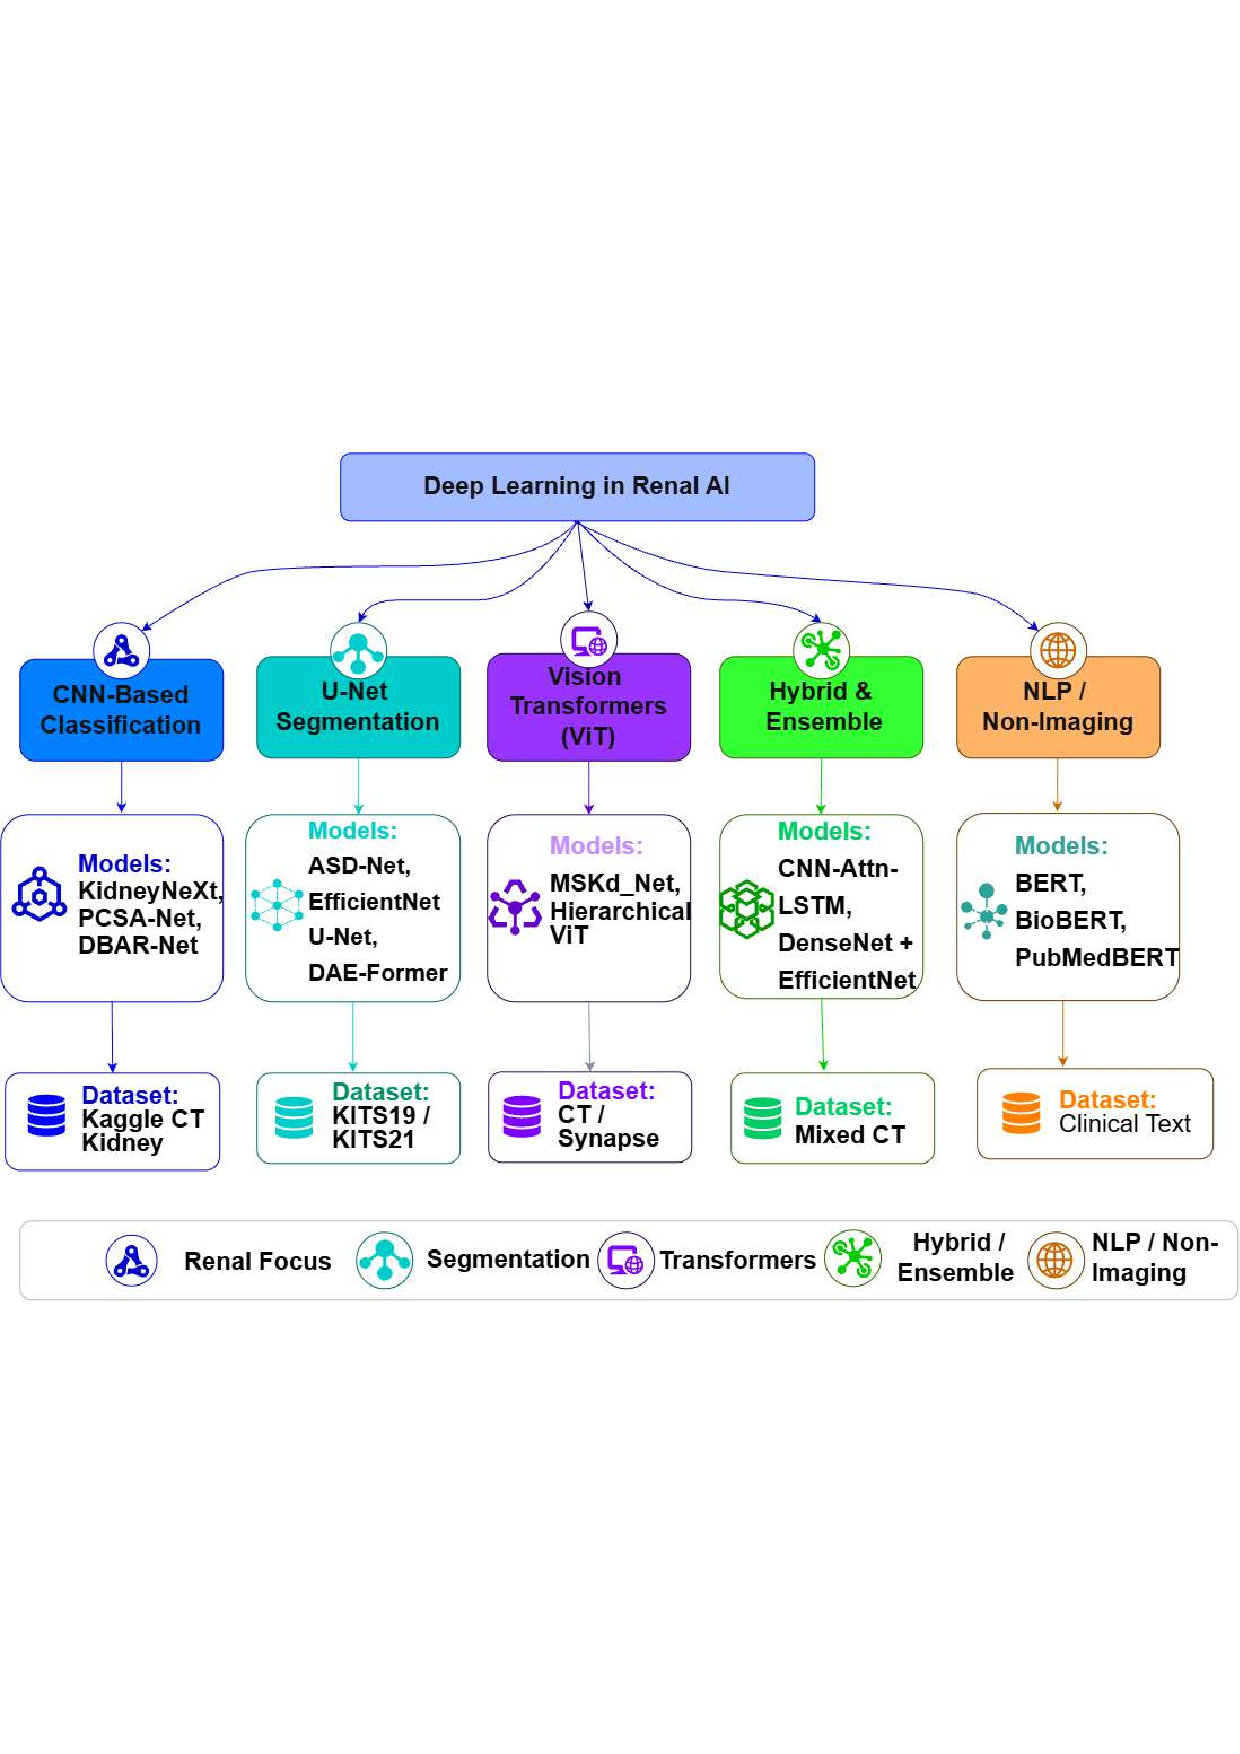
\includegraphics[width=\textwidth]{images/taxonomy_tree.pdf}
\caption{Taxonomy of deep learning architectures utilized in renal disease diagnosis, categorized by foundational feature-extraction mechanisms and their functional application.}
\label{fig:taxonomy}
\end{figure*}

\subsection{Convolutional Neural Networks (CNNs)}
CNNs remain the foundational backbone of medical image analysis due to their inherent translation invariance and efficiency in extracting localized spatial hierarchies. Within renal applications, they are primarily deployed across two functional domains.

\textbf{3D Volumetric Segmentation:} For spatial boundary mapping, the U-Net architecture and its 3D variants have dominated benchmark leaderboards. The symmetric encoder-decoder structure effectively recovers spatial resolution lost during downsampling~\cite{abdelrahman2022deep}. Recent optimizations focus on structurally modifying this core. For instance, the ASD-Net introduces an asymmetric spatial-channel convolution module to better capture irregular tumor boundaries~\cite{ji2024asdnet}, while other frameworks integrate Convolutional Block Attention Modules (CBAM) to suppress background parenchymal noise and highlight critical regions of interest~\cite{gohil2024kidney}.

\textbf{Rapid Triage Classification:} For multi-class classification, lightweight CNNs are prioritized for their high-throughput inference capabilities. Beyond these specialized boundary-mapping networks, numerous studies have successfully deployed traditional, lightweight CNN variants and ensemble methods to establish foundational diagnostic baselines for general renal abnormality detection \cite{alzubi2022kidney, bhandari2023lightweight, rathva2025ensemble, tarul2025empirical, pimpalkar2025fine, abdelrahman2023efficientnet, zhao2023automatic, chen20215d}. Architectures like KidneyNeXt leverage pyramid channel and spatial attention networks to achieve rapid diagnostic triage on standard clinical hardware, efficiently categorizing 2D axial slices into normal, cyst, tumor, or stone classifications~\cite{alqahtani2025kidneynext}.

\subsection{Vision Transformers (ViTs)}
Despite their success, CNNs are fundamentally limited by their localized receptive fields. They struggle to model long-range global dependencies—such as the spatial relationship between a multi-focal renal cell carcinoma and the broader urinary tract. 

\textbf{Global Context Modeling:} Vision Transformers address this limitation by treating images as sequences of flattened patches, applying self-attention mechanisms to weigh the global context of the entire scan simultaneously~\cite{islam2022vision}. Pure attention networks allow the model to understand holistic anatomical relationships.

\textbf{Patch-Based Multi-Scale ViTs:} Frameworks utilizing Swin Transformers attempt to reintroduce a degree of spatial hierarchy into the attention mechanism. However, pure Transformer models remain notoriously data-hungry and computationally expensive, often requiring massive pre-training datasets that are scarce in specialized medical domains. 

\subsection{Hybrid CNN-Transformer Architectures}
To bridge the gap between local precision and global contextual awareness, the current state-of-the-art has converged on Hybrid CNN-Transformer architectures. These models leverage CNN encoders to extract fine-grained, high-resolution local features and utilize Transformer modules to capture global semantic relationships.

\textbf{Cascaded Fusion:} Several notable frameworks highlight this synthesis through sequential processing. The H2Former introduces a cascaded hybrid network that continuously passes CNN and Transformer representations back and forth, achieving superior performance on complex medical image segmentation tasks~\cite{he2023h2former}.

\textbf{Dual Attention \& Routing:} Other architectures focus on optimizing the attention bottleneck. The DAE-Former utilizes a dual attention-guided efficient Transformer to provide multi-organ contouring with highly accurate spatial mapping~\cite{azad2023daeformer}. More recently, architectures like BRAU-Net++ have integrated Bi-Level Routing Attention into a U-shaped topology, significantly reducing the quadratic computational complexity of traditional self-attention while maintaining state-of-the-art Dice scores on renal benchmarks~\cite{lan2024braunet}.

By fusing these modalities, hybrid networks represent the most promising computational foundation for the unified clinical pipelines required in modern nephrology.